
\documentclass[11pt,twoside]{article}
\usepackage[utf8]{inputenc}
\usepackage[T1]{fontenc}
\usepackage{outlines}
\usepackage{float}
\usepackage{listings}
\usepackage{alloy-style}

%Page margins, header and footer positions
\usepackage{geometry}
 \geometry{
 a4paper,
 total={210mm,297mm},
 left=25mm,
 right=25mm,
 top=30mm,
 bottom=25mm,
 headsep=7mm}

\interfootnotelinepenalty=10000

%To display filling dots in the TOC for all entries
\usepackage[titles]{tocloft}
\renewcommand{\cftsecleader}{\cftdotfill{\cftdotsep}}

%Define new header and footer style
\usepackage{fancyhdr}

\pagestyle{fancy}
\fancyhf{}
\lhead{\color{Gray}{\small{Cuzzucoli Sergio, De Dominicis Daniele}}}
\lfoot{\textcolor{Gray}{\small{Copyright © 2019, Cuzzucoli Sergio, De Dominicis Daniele – All rights reserved}}}
\rfoot{\textcolor{Gray}{\thepage}}
\renewcommand{\headrulewidth}{0pt}

%PACKAGES
\usepackage{wasysym}
\usepackage{pifont}

\newcommand{\supported}{\ding{52}\xspace}
\newcommand{\unsupported}{\ding{55}\xspace}
\newcommand{\partsupported}{\textcolor{black!40}{\ding{52}}\xspace}
\newcommand{\lowsupported}{\textcolor{black!20}{\ding{52}}\xspace}
\newcommand{\unknowsupported}{\textbf{?}\xspace}

%Font: Times
\usepackage{times}
%Change monospaced font
\renewcommand{\ttdefault}{lmtt}

%tables
\usepackage{tabu}
\usepackage{tabularx}
\usepackage{ltablex}
\usepackage{longtable}
\usepackage{float} % To allow the use of H modifier in long tables

%landscape mode
\usepackage{pdflscape}
\usepackage{rotating}
\usepackage{caption}

%make landscape mode be sensitive to even and odd pages
%start
\def\myrotate{\ifodd\c@page\else-\fi 90}
\makeatletter
\global\let\orig@begin@landscape=\landscape%
\global\let\orig@end@landscape=\endlandscape%
\gdef\@true{1}
\gdef\@false{0}
\gdef\landscape{%
    \global\let\within@landscape=\@true%
    \orig@begin@landscape%
}%
\gdef\endlandscape{%
    \orig@end@landscape%
    \global\let\within@landscape=\@false%
}%
\@ifpackageloaded{pdflscape}{%
    \gdef\pdf@landscape@rotate{\PLS@Rotate}%
}{
    \gdef\pdf@landscape@rotate#1{}%
}
\let\latex@outputpage\@outputpage
\def\@outputpage{
    \ifx\within@landscape\@true%
        \if@twoside%
            \ifodd\c@page%
                \gdef\LS@rot{\setbox\@outputbox\vbox{%
                    \pdf@landscape@rotate{-90}%
                    \hbox{\rotatebox{90}{\hbox{\rotatebox{180}{\box\@outputbox}}}}}%
                }%
            \else%
                \gdef\LS@rot{\setbox\@outputbox\vbox{%
                    \pdf@landscape@rotate{+90}%
                    \hbox{\rotatebox{90}{\hbox{\rotatebox{0}{\box\@outputbox}}}}}%
                }%
            \fi%
        \else%
            \gdef\LS@rot{\setbox\@outputbox\vbox{%
                \pdf@landscape@rotate{+90}%
                \hbox{\rotatebox{90}{\hbox{\rotatebox{0}{\box\@outputbox}}}}}%
            }%
        \fi%
    \fi%
    \latex@outputpage%
}
\makeatother
%end

%graphics
\usepackage{graphicx}
\usepackage[dvipsnames, table]{xcolor}
%If you upload images from PC, you need to insert code for the path here (different for Windows and Unix OS)

%References
%\usepackage{xpatch}
%\usepackage[backend=biber, style=numeric, citestyle=numeric, sorting=none]{biblatex}
%\addbibresource{main.bib}

%Other
\usepackage{ifthen}
\usepackage{xspace}
\usepackage{enumitem}
\usepackage{amssymb}
\usepackage[pdftex, colorlinks]{hyperref}
\newcommand{\comment}[1]{{\color{Red}$\blacktriangleright$ Comment: #1 $\blacktriangleleft$}}


% Some utilities\ldots
\usepackage{soul}
\usepackage{tikz}

\usetikzlibrary{calc}
\usetikzlibrary{decorations.pathmorphing}


\makeatletter

\newcommand{\defhighlighter}[3][]{%
  \tikzset{every highlighter/.style={color=#2, fill opacity=#3, #1}}%
}

\defhighlighter{yellow}{.5}

\newcommand{\highlight@DoHighlight}{
  \fill [ decoration = {random steps, amplitude=1pt, segment length=15pt}
        , outer sep = -15pt, inner sep = 0pt, decorate
       , every highlighter, this highlighter ]
        ($(begin highlight)+(0,8pt)$) rectangle ($(end highlight)+(0,-3pt)$) ;
}

\newcommand{\highlight@BeginHighlight}{
  \coordinate (begin highlight) at (0,0) ;
}

\newcommand{\highlight@EndHighlight}{
  \coordinate (end highlight) at (0,0) ;
}

\newdimen\highlight@previous
\newdimen\highlight@current

\DeclareRobustCommand*\highlight[1][]{%
  \tikzset{this highlighter/.style={#1}}%
  \SOUL@setup
  %
  \def\SOUL@preamble{%
    \begin{tikzpicture}[overlay, remember picture]
      \highlight@BeginHighlight
      \highlight@EndHighlight
    \end{tikzpicture}%
  }%
  %
  \def\SOUL@postamble{%
    \begin{tikzpicture}[overlay, remember picture]
      \highlight@EndHighlight
      \highlight@DoHighlight
    \end{tikzpicture}%
  }%
  %
  \def\SOUL@everyhyphen{%
    \discretionary{%
      \SOUL@setkern\SOUL@hyphkern
      \SOUL@sethyphenchar
      \tikz[overlay, remember picture] \highlight@EndHighlight ;%
    }{%
    }{%
      \SOUL@setkern\SOUL@charkern
    }%
  }%
  %
  \def\SOUL@everyexhyphen##1{%
    \SOUL@setkern\SOUL@hyphkern
    \hbox{##1}%
    \discretionary{%
      \tikz[overlay, remember picture] \highlight@EndHighlight ;%
    }{%
    }{%
      \SOUL@setkern\SOUL@charkern
    }%
  }%
  %
  \def\SOUL@everysyllable{%
    \begin{tikzpicture}[overlay, remember picture]
      \path let \p0 = (begin highlight), \p1 = (0,0) in \pgfextra
        \global\highlight@previous=\y0
        \global\highlight@current =\y1
      \endpgfextra (0,0) ;
      \ifdim\highlight@current < \highlight@previous
        \highlight@DoHighlight
        \highlight@BeginHighlight
      \fi
    \end{tikzpicture}%
    \the\SOUL@syllable
    \tikz[overlay, remember picture] \highlight@EndHighlight ;%
  }%
  \SOUL@
}

\makeatother

% Common abbrev. are set as commands to ensure proper spacing after the dot
\RequirePackage{xspace}
\newcommand{\ie}{i.e.\@\xspace}
\newcommand{\aka}{a.k.a.\@\xspace}
\newcommand{\Ie}{I.e.\@\xspace}
\newcommand{\cf}{cf.\@\xspace}
\newcommand{\Cf}{Cf.\@\xspace}
\newcommand{\eg}{e.g.\@\xspace}
\newcommand{\Eg}{E.g.\@\xspace}
\newcommand{\etal}{et al.\@\xspace}
\newcommand{\etc}{etc.\@\xspace}
\newcommand{\wrt}{w.r.t.\@\xspace}
\newcommand{\Wrt}{W.r.t.\@\xspace}



\date{}


\begin{document}


\begin{titlepage}
	\centering
	
\includegraphics[width=\textwidth]{Images/PolimiLogo}\par\vspace{1cm}
	{\scshape\Huge\textbf{SafeStreets}\par}
	\vspace{1cm}
	{\scshape\Large Requirements Analysis and Specification Document\par}
	\vspace{2cm}
	{\scshape\Large\emph{Sergio Cuzzucoli}\\ \emph{Daniele De Dominicis}\par}
	\vspace{4cm}
	{\scshape\normalsize{10 November,2019}}

\end{titlepage}

%Define deliverable specific info
%Replace cell contents where needed
\begin{table}[h!]
\begin{tabu} to \textwidth { X[0.3,r,p] X[0.7,l,p] }
\hline

\textbf{Deliverable:} & RASD\\
\textbf{Title:} & Requirement Analysis and Verification Document \\
\textbf{Authors:} & Cuzzucoli Sergio , De Dominicis Daniele \\
\textbf{Version:} & 1.0 \\ 
\textbf{Date:} & 10-November-2019  \\
\textbf{Download page:} & \href{https://github.com/Danielededo/CuzzucoliDeDominicis.git}{https://github.com/Danielededo/CuzzucoliDeDominicis.git} \\
\textbf{Copyright:} & Copyright © 2019, Cuzzucoli Sergio, De Dominicis Daniele – All rights reserved \\
\hline
\end{tabu}
\end{table}




\setcounter{page}{2}


%------------------------------------------------------------------------------------------------------------------------------------------------
\newpage
\addcontentsline{toc}{section}{Table of Contents}
\tableofcontents
\newpage
%\addcontentsline{toc}{section}{List of Figures}
%\listoffigures
%\addcontentsline{toc}{section}{List of Tables}
%\listoftables

%------------------------------------------------------------------------------------------------------------------------------------------------
\clearpage
{\section{Introduction}}
\label{sect:introduction}
\subsection{Purpose}

Safestreet is the name of an application aiming to offer principally the possibility to signal traffic or parking violation via the internet to public authorities.
This document aims to outline the functioning of said app, providing a deep insight of the software and supporting the stakeholders.

Safestreet offers, as a basic functionality, the possibility to fill in a form detailing one of the possible violations (e.g. illegal parking) to every single user. The application gives its users the possibility to compile a form complete with a brief description of the wrongdoing and several additional information. Said information consists of the position of the user at the time of the report (street name) and some pictures, to be attached to the form itself in some way (for example using the smartphone on which the app is installed). The form can then be either approved and investigated or discarded by the public authorities working at the interested area (in both cases the user is warned of the end result of their report). At the same moment Safestreet stores data received by those warnings and computes them to highlight areas in which a violation is most likely to occur, or to show which type of vehicle tends to be associated with different wrongdoings.

In addition to what is written above, the data mined from the warnings can be crossed with that offered by the municipality. If a specific part of the city presents an alarming number of reports it may mean that the infrastructures provided to the population are inadequate or that part of the citizens (especially the weaker ones such as bikers or the elderly) is not preserved enough, thus some suggestions can be made to the authorities in order to avoid further inconveniences.

\subsection{Goals}

The goals set are expressed from the point of view of the S2B:

\begin{itemize}
\item [G1]{The application has to store all the information about violations sent to it, until a ticket is either dropped or accepted by an authority}
\item [G2]{The system must accepts reports issued from every part of the covered area }
\item [G3]{The system must allow authorities to access reports in every part of the covered area}
\item [G4]{The application allows users and authorities to mine information on the system}
\item [G5]{The application identifies unsafe areas crossing its informations with those offered by the municipality}
\item [G6]{The application suggests possible solution to problems perceived after the crossing of information}
\end{itemize}

\begin{figure}

\includegraphics[width=\textwidth]{Images/Templates/icon-safestreets.PNG}
\end{figure}

\subsection{Scope}

Safestreet poses itself as an intermediate between users and authorities.\\
%Users must be equipped with smartphones provided with camera and GPS tracker.\\
Users file reports via the mobile app. 
Authorities (e.g. a police person) examine the report and can discard it or investigate it, leading to a positive result (fine or warning) or negative one (no violation revealed).\\
Saved reports are analyzed and data extracted by them can be consulted both by users and authorities (at different levels).
If the municipality offers data about accidents, they are crossed with those obtained by SafeStreets and suggestion based on them are made. Data is visible to everyone (at different levels).

\subsubsection{World Phenomena}

\begin{itemize}

\item \textbf{Broken rules}: Drivers commit violations

\item \textbf{Observation}: Citizens observe possible violations

\item \textbf{Inspection}: Authorities inspect possible violations 

\item \textbf{Unfortunate events}: Accidents happen

\end{itemize}

\subsubsection{Machine Phenomena}

\begin{itemize}

\item \textbf{DBMS}: All operations to retrieve or store data

\item \textbf{Classification}: Statistics are redacted and streets ordered accordingly

\end{itemize}

\subsubsection{Shared Phenomena}

\subsubsection*{Controlled by the world and observed by the machine}

\begin{itemize}

\item \textbf{Login}: Citizens undergo the SMS procedure and authorities login using ID and password

\item \textbf{File report}: Citizens file a report

\item \textbf{Inspect report}: Authorities discard or complete a report

\end{itemize}

\subsubsection*{Controlled by the machine and observed by the world}

\begin{itemize}

\item \textbf{Show data of violations}: Violations are listed and acessible by everyone

\item \textbf{Show data of accidents}: Accidents are listed and acessible by everyone

\item \textbf{Show suggestions}: Suggestion are made according to accidents and violations, for the authorities to see

\end{itemize}

\subsection{Definitions, Acronyms, Abbreviations}

\subsubsection{Definitions}

\begin{itemize}

\item Smartphone: Device that allows for calls together with internet connectivity and GPS tracking

\item User: Citizen who has installed Safestreet on their smartphone

\item Authority: Public official or ent that monitors the territory and mantains the order

\item Violation: Act of breaking rules of the road code

\item Accident: Violent collision involving vehicles (motorized or not) and/or animate or inanimate objects
 
\end{itemize}

\subsubsection{Acronyms}
\begin{tabular}{|l|l|}
\hline
Acronym & Meaning \\ \hline
DB & Data Base \\ \hline
DBMS & Data Base Management System \\ \hline
API & Application Program Interface \\ \hline
UI & User Interface \\ \hline
OS & Operating System \\ \hline
RASD & Requirement Analysis and Specification Document \\ \hline
GPS & Global Positioning System \\ \hline
CNN & Convolutional Neural Network \\
\hline
\end{tabular}

\subsubsection{Abbreviation}

\begin{itemize}

\item [\textbf{G.th}]: n-th Goal

\item [\textbf{D.th}]: n-th Domain Assumption

\item [\textbf{R.th}]: n-th Functional Requirement

\end{itemize}

\subsection{Reference Documents}

\begin{itemize}

\item Project assignment specifications:\cite{assignment.pdf}

\item Alloy Documentation:\cite{http://alloy.lcs.mit.edu/alloy/documentation.html}

\end{itemize}

\subsection{Document Structure}

\begin{itemize}

\item \textbf{Overall description}: a general description of the service is provided, together with a furter inspection on shared phenomena. Relevant functions of the System are explained. Finally, through the specifications of constraints, dependencies and assumptions, it is unveiled how the System is integrated in the real world.

\item \textbf{Specific requirements}: aimed to both designers and testers, all the aspects of the previous section are put into perspective. Requirements
are fully explained and divided by types and possible interactions with the System are investigated through use cases and sequence diagrams.

\end{itemize}

%------------------------------------------------------------------------------------------------------------------------------------------------
\clearpage
{\section{Overall Description}}
\label{sect:overview}
\subsection {Product Perspective}

In this paragraph we shall deepen the shared phenomena mentioned in the previous section, providing an oversight of the domain model on different levels of specification, by means of class and state diagrams.

\begin{itemize}

\item \textbf{Login (controlled by the world and observed by the machine)}: On every opening of the app, users must insert their phone number, then the code generated by the server and sent to them by SMS. Authorities enter using their ID code and password provided to them in a previous moment.

\item \textbf{File report (controlled by the world and observed by the machine)}: Users must take a photo of the violation and specify the type, position is obtained by the tracker in the phone, date and time are provided by the server, and a brief description can be attached. Nowithstanding that the system exploits computer vision and artificial intelligence to identify the license plate of the vehicle in the photos, the user must add the number to improve the accuracy of the violation.In case of incomplete identification the user is warned and invited to retake the photo (violations with no photo or incomplete plate identification are not accepted, and the user must start over). If the violation complies with all this rules, it is sent to Safestreets' DBMS.

\item \textbf{Inspect violation (controlled by the world and observed by the machine)}: Authorities have access to all the pending violations of their city. They can discard the violation (its data is erased by the DBMS) or inspect it. Exploiting Google Maps' API, they are guided to the position of the violation. The result can be either positive (the violation is verified and a fine or a warning is issued) or negative. In the former option the violation is saved on the database, in the latter one, the data is discarded.

\item \textbf{Show data of violations (controlled by the machine and observed by the world)}: All the successful violations are stored on the DB with statistics regarding every street. Streets are ordered by the number of violations committed during the previous month in decreasing orderd. Users can select a street and acknowledge the number of violation type by type, authorities see also the list of the plates of the offenders.

\item \textbf{Show data of accidents (controlled by the machine and observed by the world)}: If the \\ municipality offers data about accidents it is crossed with that of Safestreets, street by street. Streets are ordered by the number of accidents, those who have a number of accidents equal to or greater than the treshold (for example \textcolor{Red}{12}) are marked unsafe, and the most common type of violation is shown. The number of accidents can be seen by everyone.

\item \textbf{Show suggestions (controlled by the machine and observed by the world)}: Suggestion are formulated for unsafe streets based on the most common type of violation, they can be seen only by the authorities.

\end{itemize}

Following are the class and state diagrams:

%TODO

\subsection{Product Functions}

Here the most important features of the product are outlined:

\subsubsection{Data management}

Data offered by the municipality are replicated and not modified.

\subsubsection*{Data management by the users}

Users are allowed to send information about their violation on the DB but have no power over their conservation. 

\subsubsection*{Data management by the authorities}

Authorities have the power to delete (discard) a case, or to inspect it and close it, keeping it on the DB in the end. 

\subsubsection{Data Requests}

Users and authorities can retrieve information stored previously on the DB by the means of a DBMS.

\subsubsection*{Requests by the users}

Users are unable to see their previous report but can retrieve general information about violations under the form of a list of streets, ordered by the one with the greatest number of violation to the one with the smallest. Every street can be highlighted and the types of violations are ordered in a similar fashion. They can also access a list of streets with their respective number of accidents, ordered from the most unsafe street to the least unsafe one.

\subsubsection*{Requests by the authorities}

Authorities can access all the pending violations in their city. They have the same powers as the citizens but they can retrieve more info. When accessing the list of streets by violation, they are allowed to see the plates of repeated offenders of the street, from the most incorrect to the least. Upon inspection of the street, taken by the list which focuses on accidents, they are prompted with suggestions on how to improve the security of the street itself.


\subsection{Users characteristics}

\begin{itemize}

\item \textbf{User}: A citizen who has SafeStreets installed on their smartphone.

\item \textbf{Authority}: Social community workers or administrative workers who keep control of the in general,

\end{itemize}

\subsection{Assumptions, dependencies and constraints}

\subsubsection{Assumptions}

\subsubsection*{Basic Service}

\begin{itemize}

%\item \textbf{D1}: Users must be equipped with smartphones provided with camera, internet connection and GPS tracker

\item \textbf{D1}: The smartphone of the user can provide accurate location

\item \textbf{D2}: The data provided by the user is correct

\item \textbf{D3}: Internet connection is reliable

\item \textbf{D4}: The CNN is always on and ready to communicate

\item \textbf{D5}: There is no failure in communication

\item \textbf{D6}: GM is always on and ready to communicate

\item \textbf{D7}: Data storage is reliable

\end{itemize}

\subsubsection*{Advanced Funcionality}

\begin{itemize}

\item \textbf{D8}: Data offered by municipality is correct

\item \textbf{D9}: Data offered by municipality is up-to-date

\end{itemize}

\subsubsection{Dependencies}

\begin{itemize}

\item The system needs a DBMS to store and retrieve data

\item GM is provided by Google

\item CNN is provided by an external body

\end{itemize}

\subsubsection{Constraints}

\begin{itemize}

\item Users must be equipped with smartphones provided with camera, internet connection and GPS tracker

\item Authorities must be equipped with smartphones provided with camera, internet connection and GPS tracker or a computer with a working internet connection and a browser installed upon.

\item Users' smartphone mount an OS compatible with the application

\item Authorities' smartphone mount an OS compatible with the application

\item Authorities' computer has an internet browser installed upon

\end{itemize}

%------------------------------------------------------------------------------------------------------------------------------------------------
\clearpage
{\section{Specific Requirements}}
\label{sect:requirements}
%\subsection{External Interface Requirements}

\subsubsection{User Interfaces}
\begin{figure}
[H]
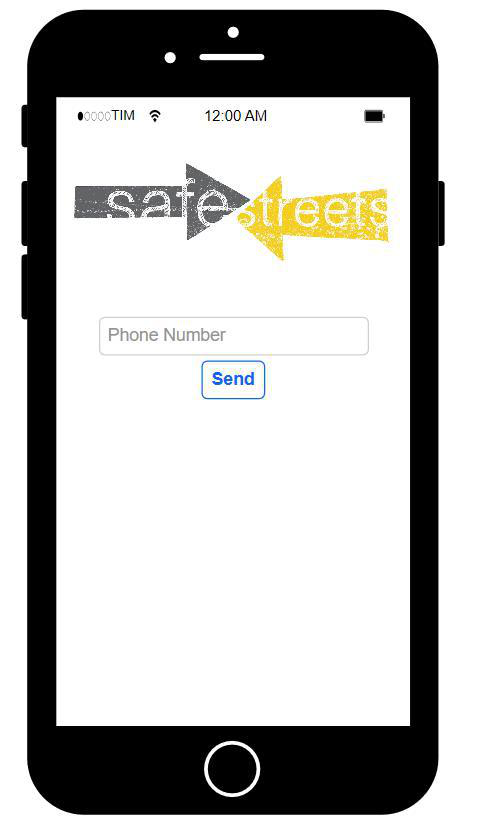
\includegraphics[scale=0.52]{Images/Templates/User/us_0.png}
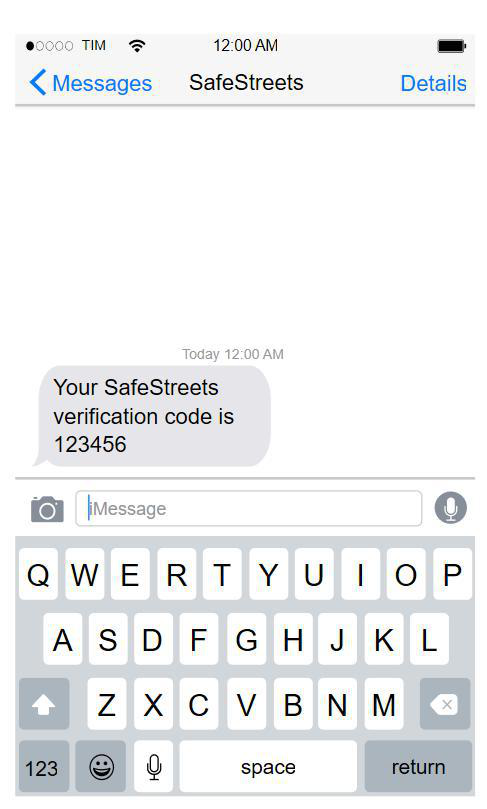
\includegraphics[scale=0.5]{Images/Templates/User/us_1.png}
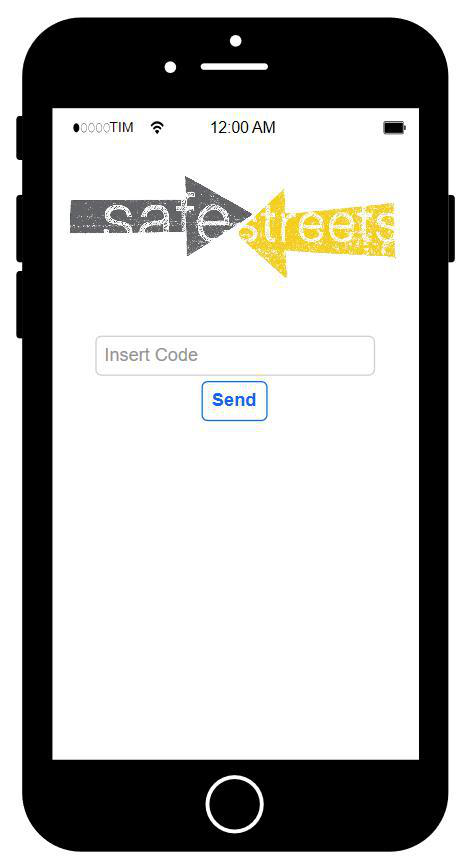
\includegraphics[scale=0.5]{Images/Templates/User/us_2.png}
\caption{\label{fig:Mockup-1}Login}
\end{figure}

\begin{figure}
[H]
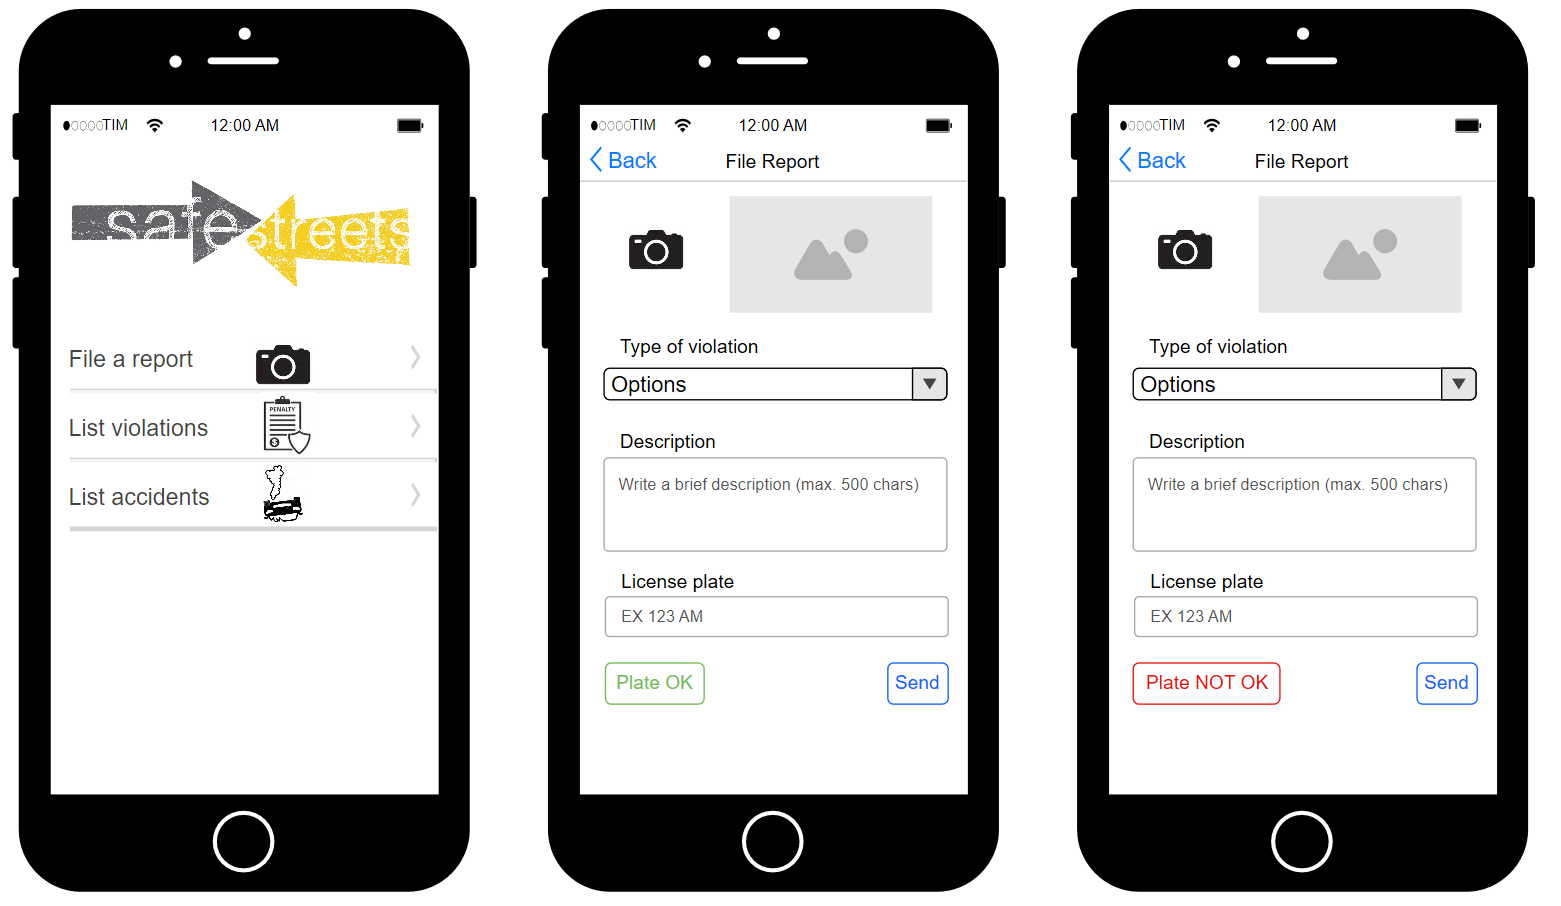
\includegraphics[scale=0.47]{Images/Templates/User/us_3.PNG}
\caption{\label{fig:Mockup-2}Menu and File Report section}
\end{figure}

\begin{figure}
[H]
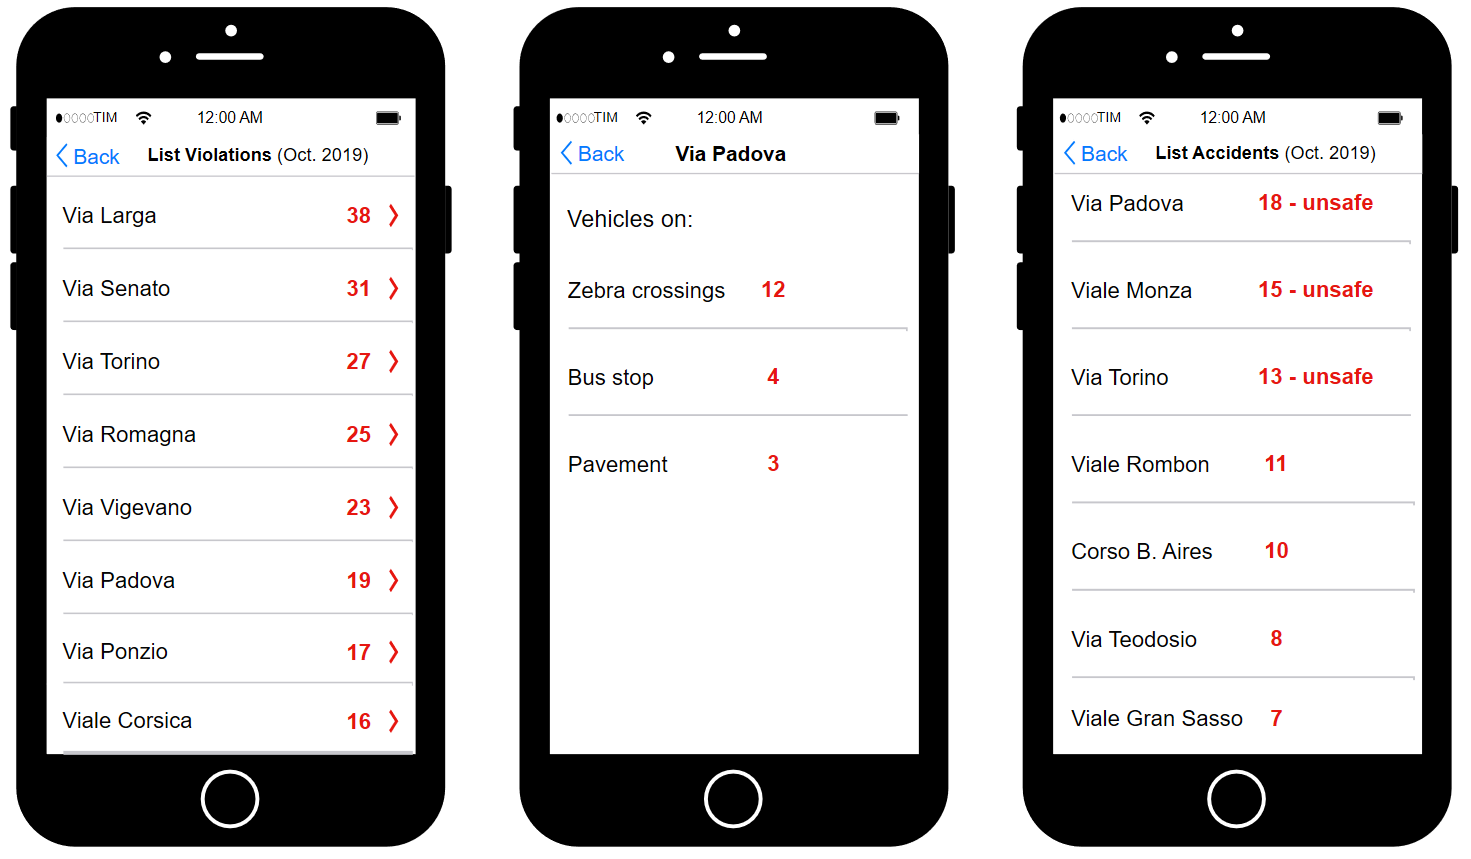
\includegraphics[scale=0.5]{Images/Templates/User/us_4.PNG}
\caption{\label{fig:Mockup-3}List Violations and List Accidents sections}
\end{figure}

\subsubsection{Authority Interfaces}
\begin{figure}
[H]
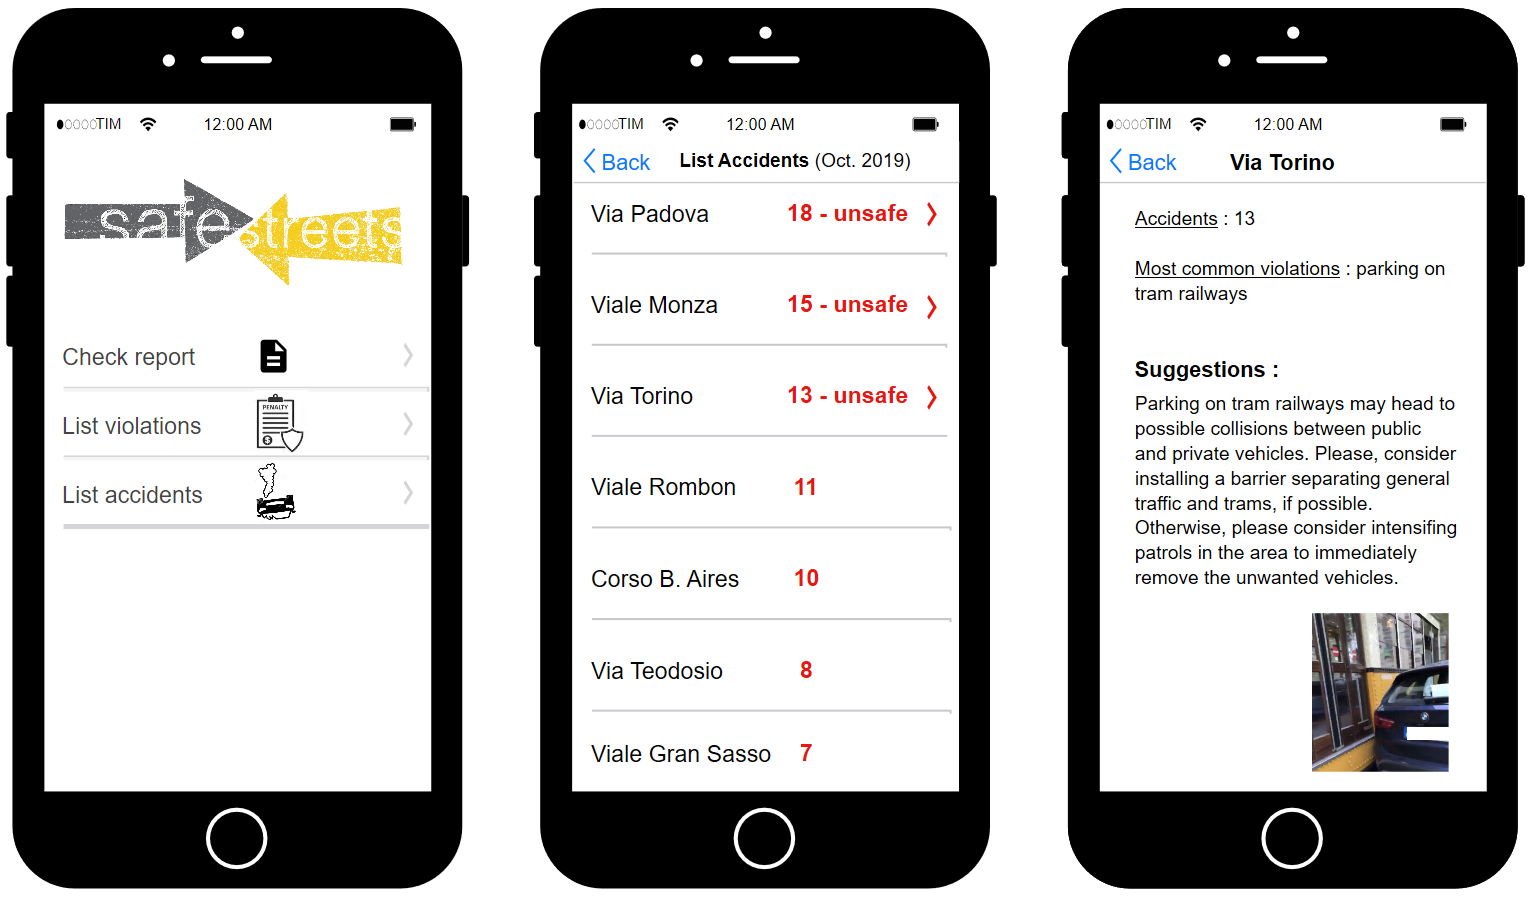
\includegraphics[scale=0.48]{Images/Templates/Authority/auth_0.PNG}
\caption{\label{fig:Mockup-4}Menu and List Accidents section}
\end{figure}

\begin{figure}
[H]
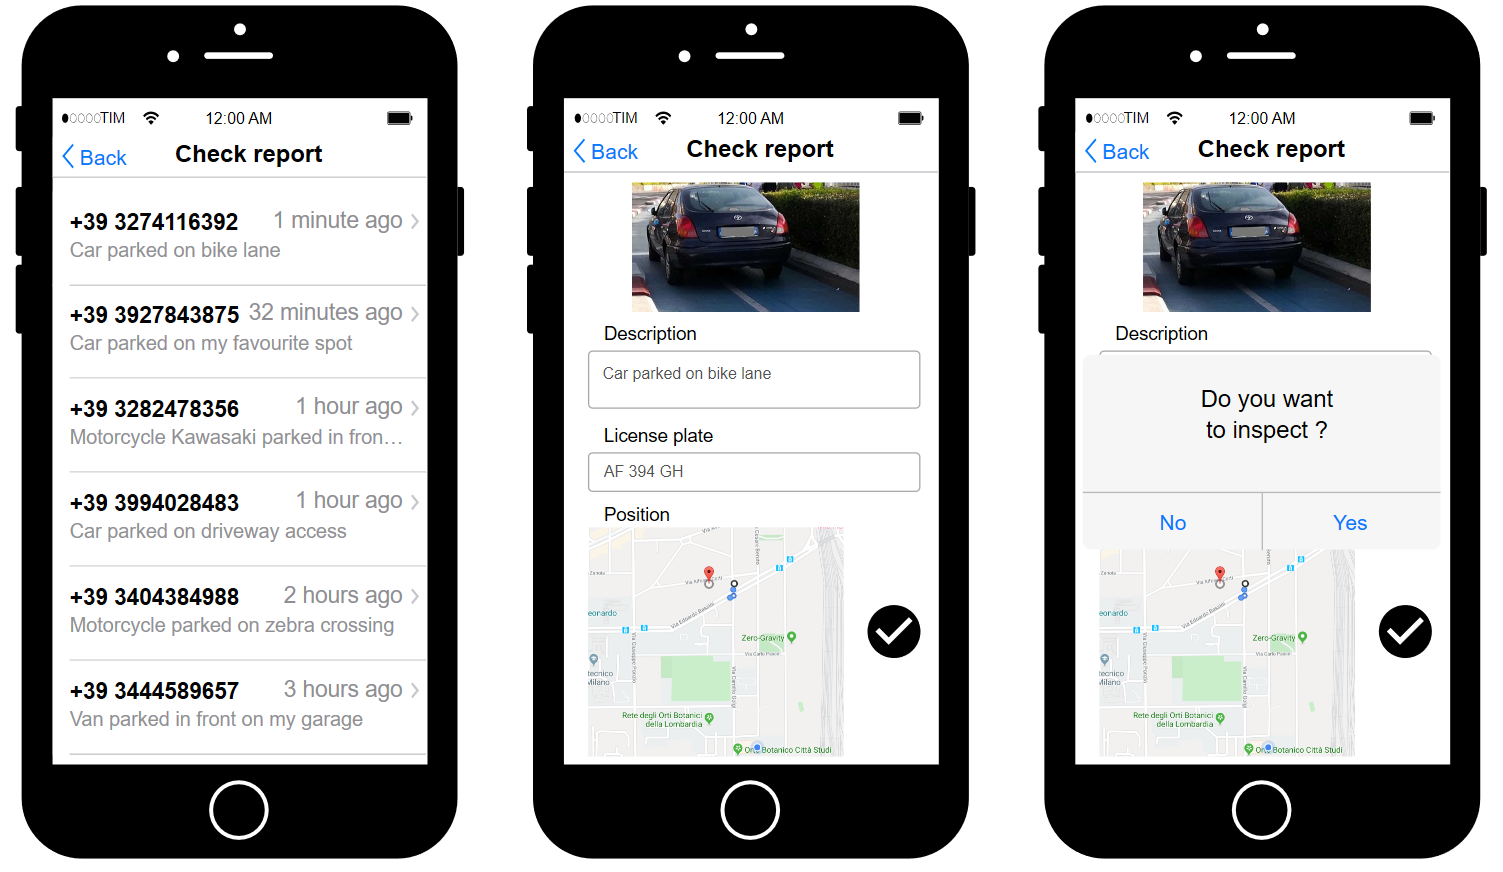
\includegraphics[scale=0.49]{Images/Templates/Authority/auth_1.PNG}
\caption{\label{fig:Mockup-5}Check Report section}
\end{figure}

\begin{figure}
[H]
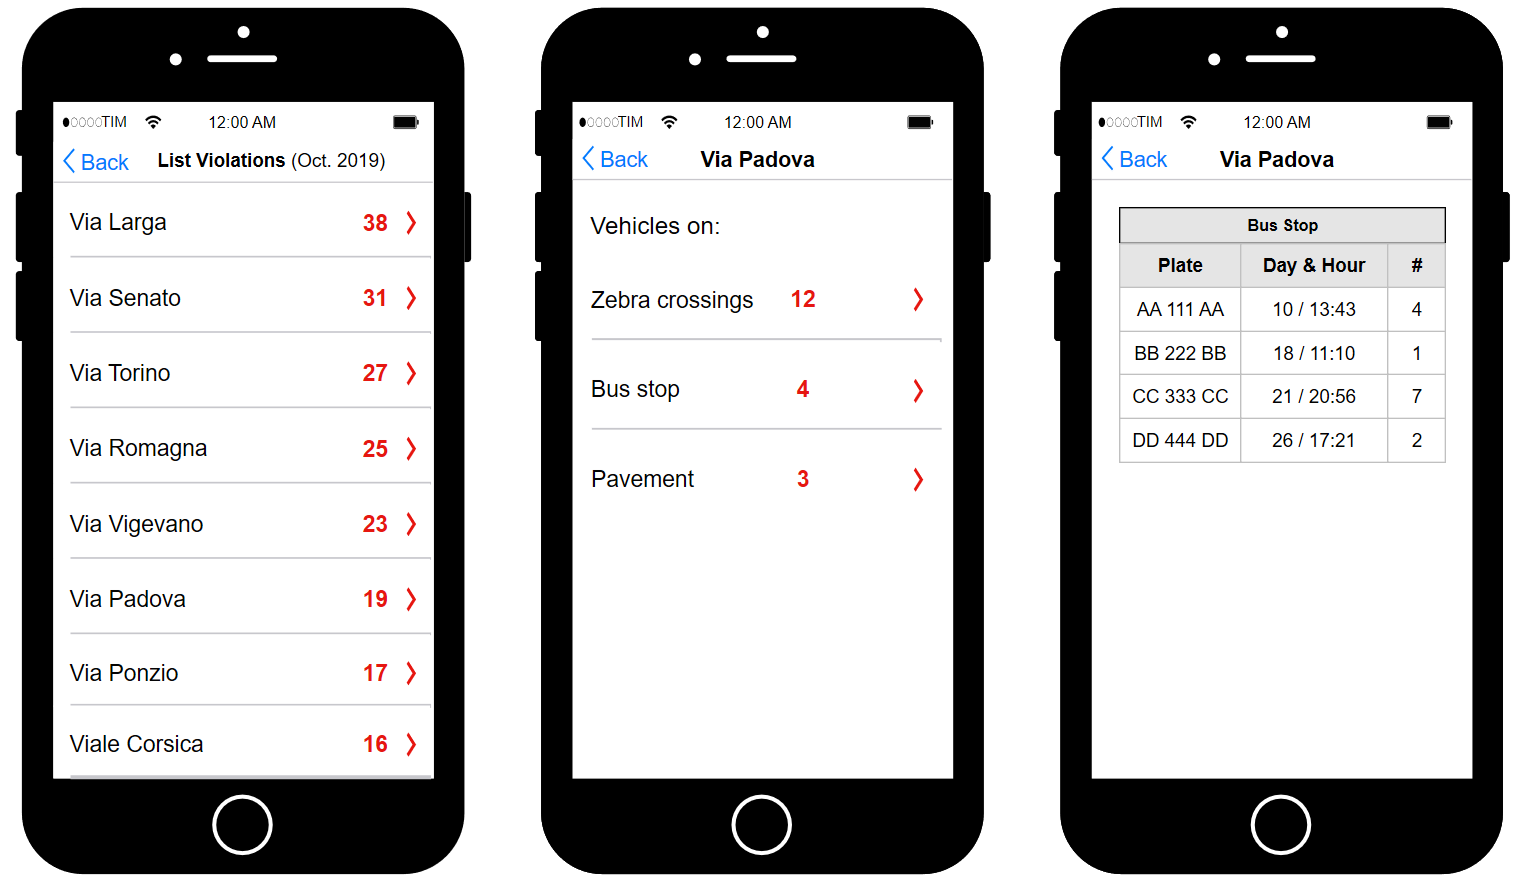
\includegraphics[scale=0.48]{Images/Templates/Authority/auth_2.PNG}
\caption{\label{fig:Mockup-6}List Violations section}
\end{figure}

\begin{figure}
[H]
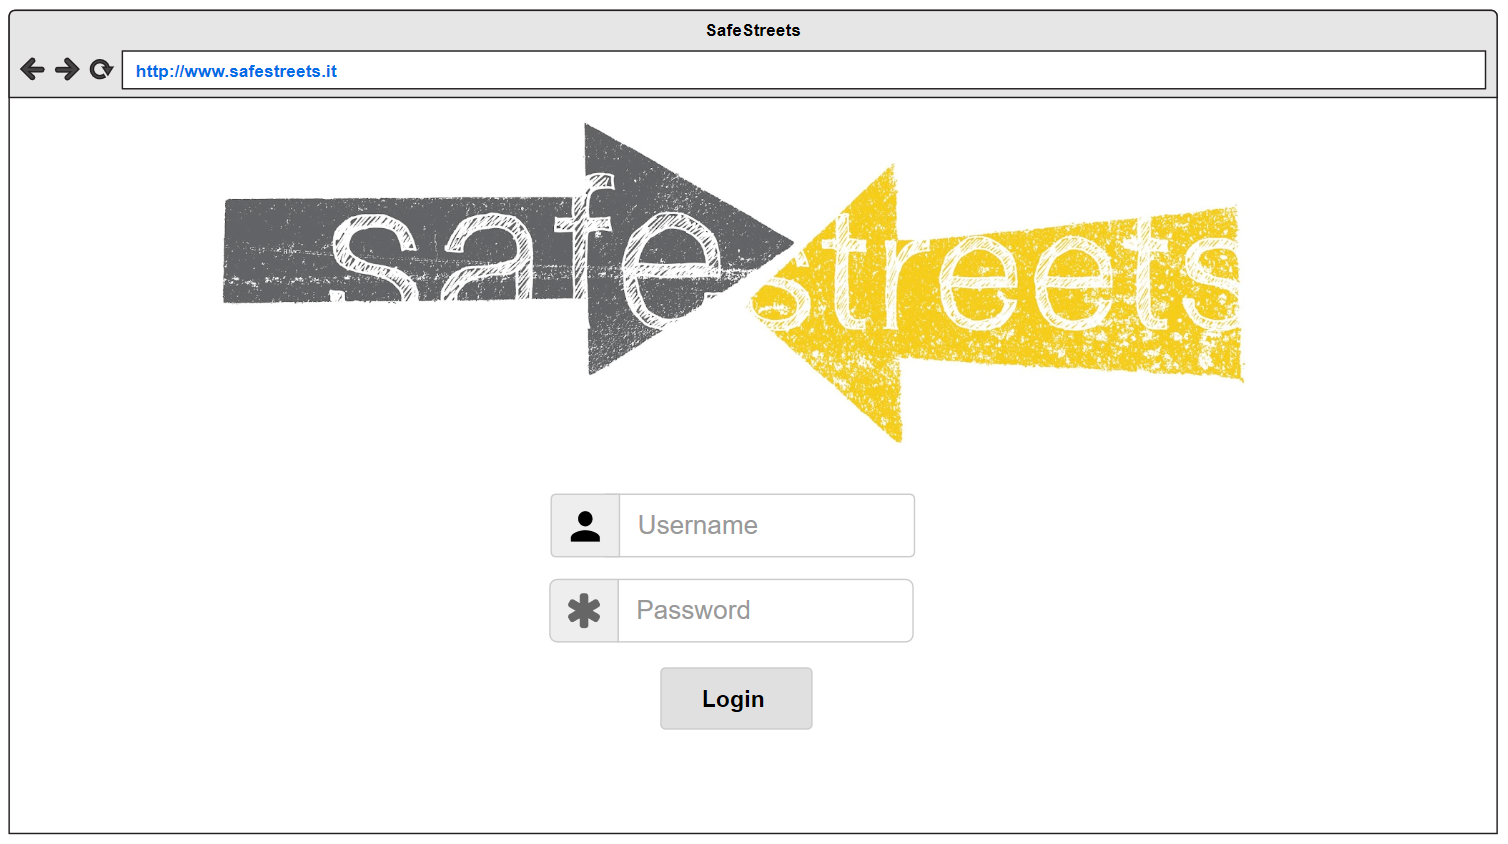
\includegraphics[scale=0.5]{Images/Templates/Authority/auth_3.PNG}
\caption{\label{fig:Mockup-7}Web Login interface}
\end{figure}

\begin{figure}
[H]
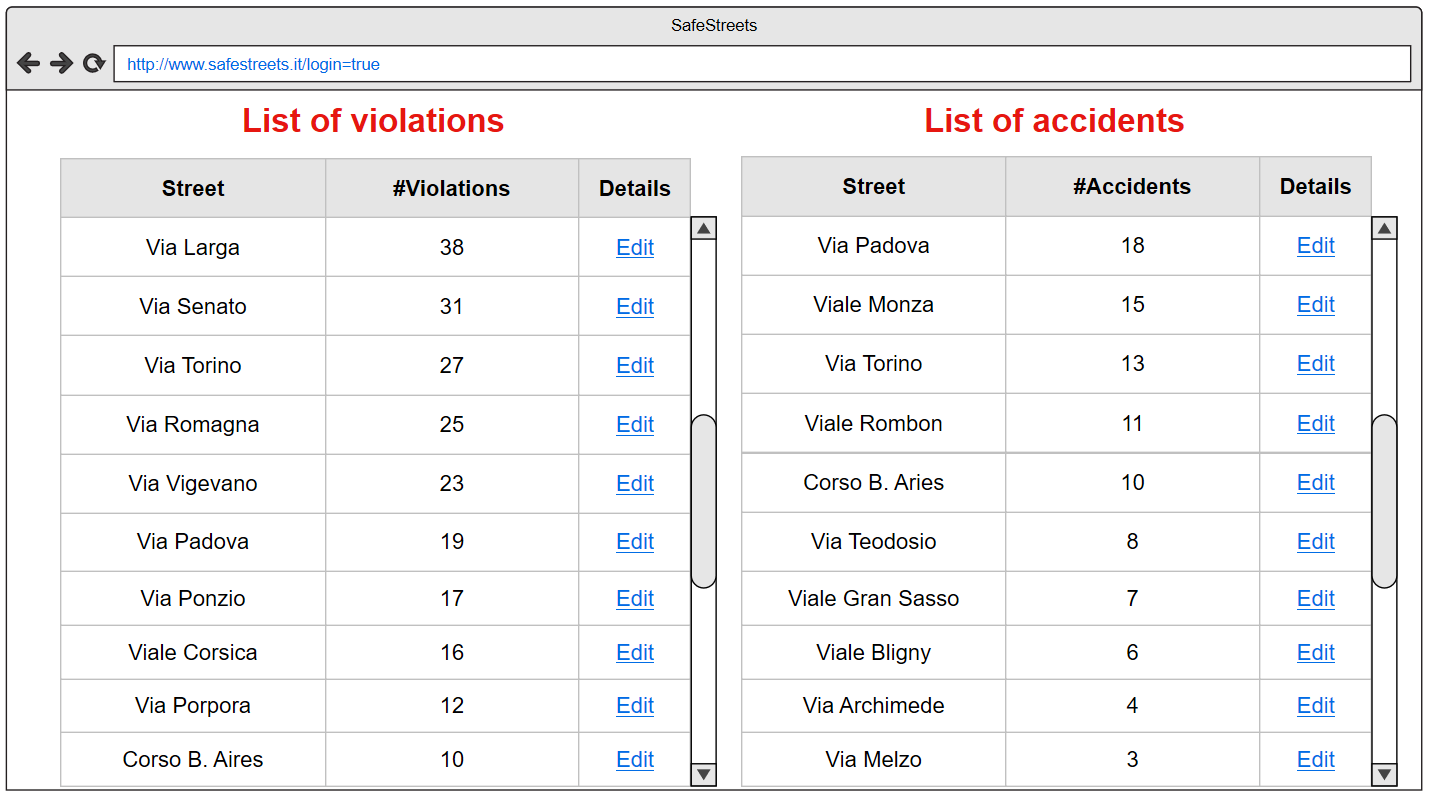
\includegraphics[scale=0.5255]{Images/Templates/Authority/auth_4.PNG}
\caption{\label{fig:Mockup-8}Web interface}
\end{figure}
\newpage

\subsubsection{Hardware Interfaces}

The application is available to those who have a smartphone with internet connection (to communicate with SafeStreet), a camera (to take photos of the violations) and a GPS tracker (to provide the position).
The web application for authorities can be accessed by any computer with a web browser.

\subsubsection{Software Interfaces}

\begin{itemize}

\item Browser
\item Web Server Application
\item Operating System: iOS, Android
\item DBMS

\end{itemize} 

\subsubsection{Communication Interfaces}

This application requires an Internet connection for the purpose of transmitting the report information, HTTPS protocol is used to transfer the data securely between the user and the DBMS.

\subsection{Functional Requirements}
\begin{outline}

\1  \textbf{G1} The application has to store all the information about violations sent to it, until a ticket is either dropped or accepted by an authority

\2 \textbf{D5}: There is no failure in communication

\2 \textbf{D7}: Data storage is reliable

\2 \textbf{R1}: Users must login with their cellphone number to send a violation


%____________________________________________________________________________

\1  \textbf{G2} The system must accepts violations issued from every part of the covered area

\2 \textbf{D1}: The smartphone of the user can provide accurate location

\2 \textbf{D3}: Internet connection is reliable

\2 \textbf{D4}: The CNN is always on and ready to communicate

\2 \textbf{D5}: There is no failure in communication

\2 \textbf{R2}: Users must be connected to the internet with their GPS enabled to use the service

%____________________________________________________________________________

 
\1  \textbf{G3} The system must allow authorities to access violations in every part of the covered area

\2 \textbf{D3}: Internet connection is reliable

\2 \textbf{D5}: There is no failure in communication

\2 \textbf{D6}: GM is always on and ready to communicate

\2 \textbf{D7}: Data storage is reliable

%____________________________________________________________________________

\1  \textbf{G4} The application allows users and authorities to mine information on the system

\2 \textbf{D3}: Internet connection is reliable

\2 \textbf{D5}: There is no failure in communication

\2 \textbf{D7}: Data storage is reliable

%____________________________________________________________________________

\1  \textbf{G5} The application identifies unsafe areas crossing its informations with those offered by the municipality

\2 \textbf{D7}: Data storage is reliable

\2 \textbf{D8}: Data offered by municipality is correct

\2 \textbf{D9}: Data offered by municipality is up-to-date


%____________________________________________________________________________

\1  \textbf{G6} The application suggests possible solution to problems perceived after the crossing of information

\2 \textbf{D2}: The data provided by the user is correct

\2 \textbf{D8}: Data offered by municipality is correct

\2 \textbf{D9}: Data offered by municipality is up-to-date

\end{outline}

\subsubsection{Use Case Diagrams}
\begin{figure}
[H]
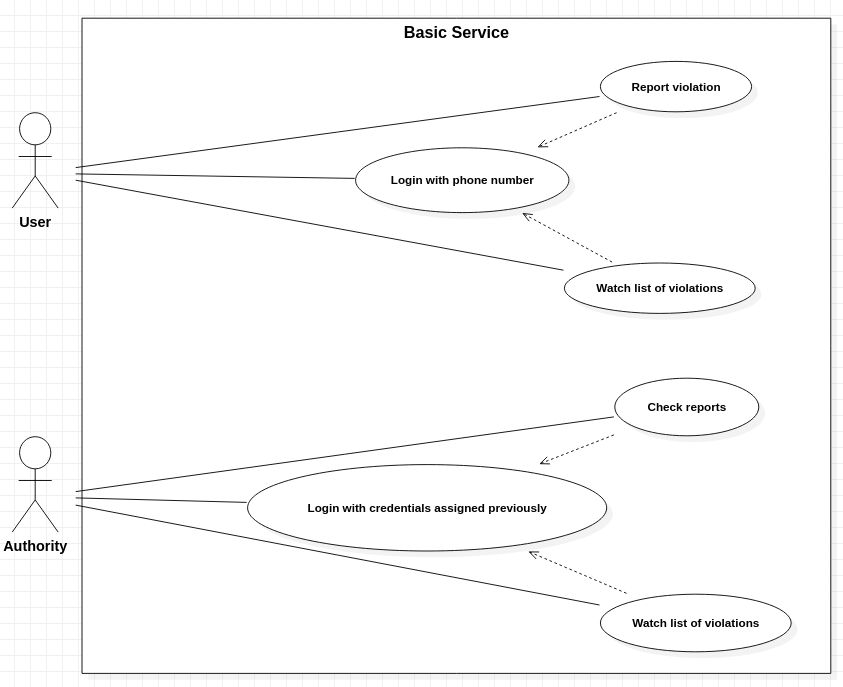
\includegraphics[width=\textwidth]{Images/Diagrams/UseCase1.png}
\caption{\label{fig:UseCase1}SafeStreets basic service use case diagram}

\end{figure}

\begin{figure}
[H]
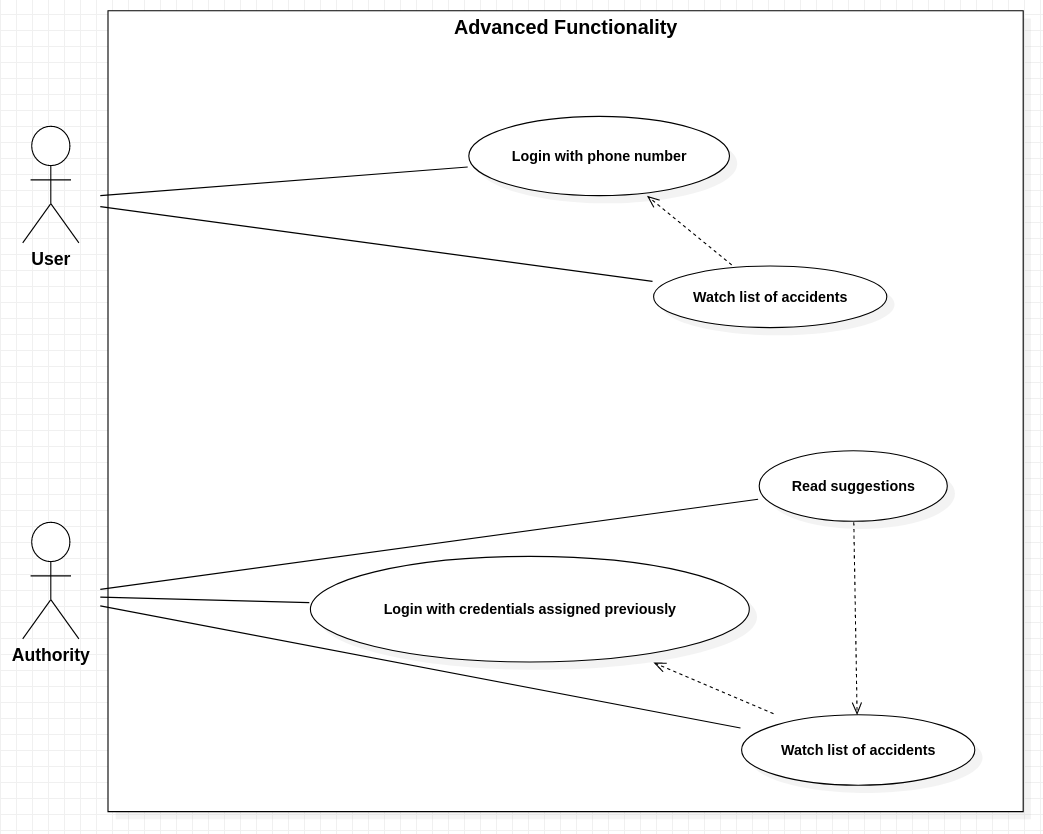
\includegraphics[width=\textwidth]{Images/Diagrams/UseCase2.png}
\caption{\label{fig:UseCase2}SafeStreets advanced functionality use case diagram}
\end{figure}

\subsubsection{Use Case Templates}

\subsubsection{Sequence Diagram}
\begin{figure}
[H]
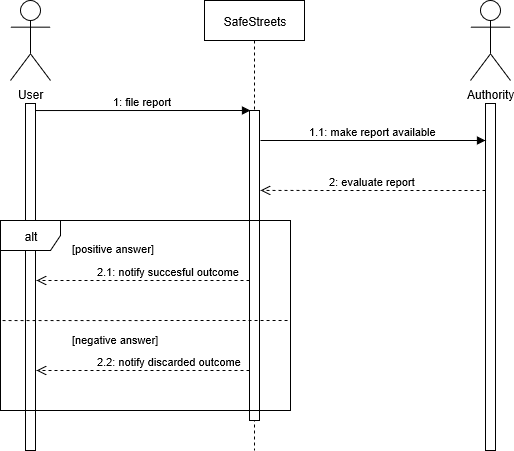
\includegraphics[width=\textwidth]{Images/Diagrams/Sequence1.png}
\caption{\label{fig:Sequence1}Lifetime of a report}
\end{figure}

\begin{figure}
[H]
\centering
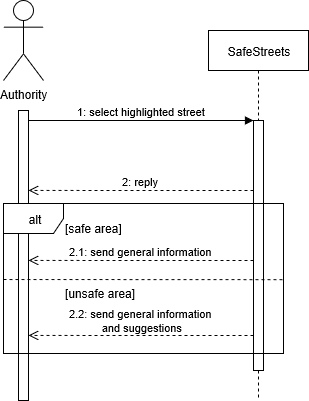
\includegraphics[scale=1]{Images/Diagrams/Sequence2.png}
\caption{\label{fig:Sequence2}Examination of accidents}
\end{figure}

%------------------------------------------------------------------------------------------------------------------------------------------------
\clearpage
{\section{Formal Analysis Using Alloy}}
\label{sect:alloy}
%Organize this section according to the rules defined in the project description. 


%------------------------------------------------------------------------------------------------------------------------------------------------
\clearpage
{\section{Effort Spent}}
\label{sect:effort}
%
\centering{

\begin{tabular}{|l|l|l|}

\hline

\textsc{Date} & \textsc{Task} & \textsc{Hours} \\

\hline

\end{tabular}

Cuzzucoli Sergio 

\vspace{2cm}

\begin{tabular}{|l|l|l|}

\hline

\textsc{Date} & \textsc{Task} & \textsc{Hours} \\

\hline

\end{tabular}

De Dominicis Daniele

}


%------------------------------------------------------------------------------------------------------------------------------------------------
\clearpage
\addcontentsline{toc}{section}{References}
\bibliographystyle{plain}
\bibliography{main}
%------------------------------------------------------------------------------------------------------------------------------------------------

\end{document}
